\chapter{Analisi dei Requisiti}
\label{cap:analisi_requisiti}




\section{Multiple Description Coding}


Un \emph{codec} è un dispositivo (hardware o software) in grado di codificare e
decodificare alcune informazioni in un formato di rappresentazione particolare.
In genere il termine è usato in relazione a flussi multimediali (audio/video)
processati tramite un elaboratore elettronico. Esistono molti modelli per la
realizzazione di codec; il più diffuso in questo momento, per lo streaming di
flussi multimediali, è il Modello \emph{Layered}\footnote{Il Modello
\emph{Layered} è alla base di codec come MPEG e derivati (MP3, DivX, ecc.)}. Un
nuovo modello (\emph{Multiple Descriptions}) ha fatto da qualche anno la sua
comparsa: prevede una diversa organizzazione delle informazioni, che sembra più
indicata per reti con una alta probabilità d'errore e senza supporto per la
Quality-of-Service.


\subsection{Modello \emph{Layered}}
Il Modello \emph{Layered} prevede che i codec debbano suddividere un flusso
multimediale (vedi Figura \ref{fig:modello_layered}) in:
\begin{itemize}
  \item uno ``strato base'' (\emph{Base Layer})
  \item diversi ``strati avanzati'' (\emph{Enhanced Layers}) 
\end{itemize}

\begin{figure}[hb]
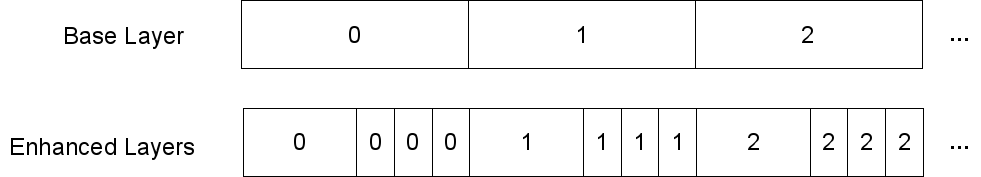
\includegraphics[width=0.90\textwidth]{../images/modello_layered.png}
\label{fig:modello_layered}
\caption{Modello Layered}
\end{figure}

Il principio è che gli \emph{Enhanced Layers}, essendo non necessari, possano
essere inviati solo a chi ne fa specifica richiesta, per aumentare la
qualità del flusso.


Questo tipo di approccio, anche se molto diffuso, presenta alcune problematiche.
I flussi multimediali generalmente vengono trasmessi tramite reti che non
garantiscono il trasporto privo di errori (\emph{best effort}). Ogni pacchetto
inviato ha una certa probabilità di giungere a destinazione corrotto, oppure di
non arrivare affatto. Nel Modello \emph{Layered} questi errori potrebbero
intaccare in pacchetto di un \emph{Enhanced Layer} oppure di un \emph{Base
Layer}: nel primo caso si avrà solo una piccola perdita di qualità (vedi Figura
\ref{fig:modello_layered_errori1}, mentre nel secondo caso si avranno
conseguenze potenzialmente disastrose, come la perdita di continuità nel flusso
(vedi Figura \ref{fig:modello_layered_errori2}. Se il flusso non è real-time, è
possibile chiedere nuovamente alla sorgente il frammento danneggiato: un \emph{Base Layer} però contiene solitamente molte più informazioni, quindi è più oneroso ritrasmetterlo.
Infine, gli \emph{Enhanced Layers} hanno un senso solo se rapportati al loro
strato base, quindi è necessario far si che giungano in istanti di tempo vicini:
altrimenti sarebbero inutili.

\begin{figure}[h]
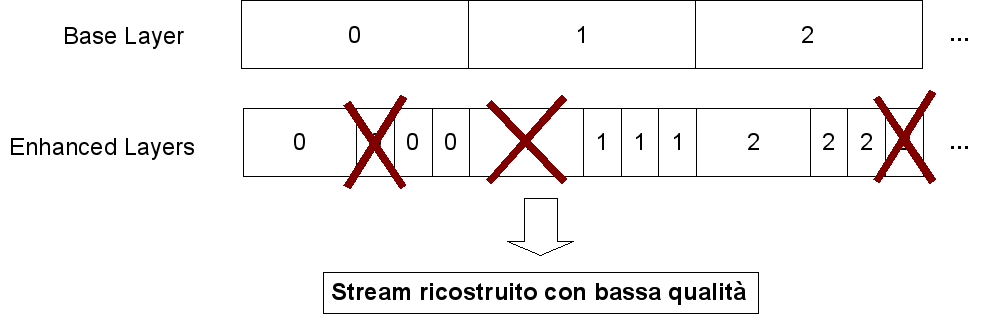
\includegraphics[width=0.90\textwidth]{../images/modello_layered_errori1.png}
\label{fig:modello_layered_errori1}
\caption{Modello Layered: perdita di un ``Enhanced Layer''}
\end{figure}

\begin{figure}[h]
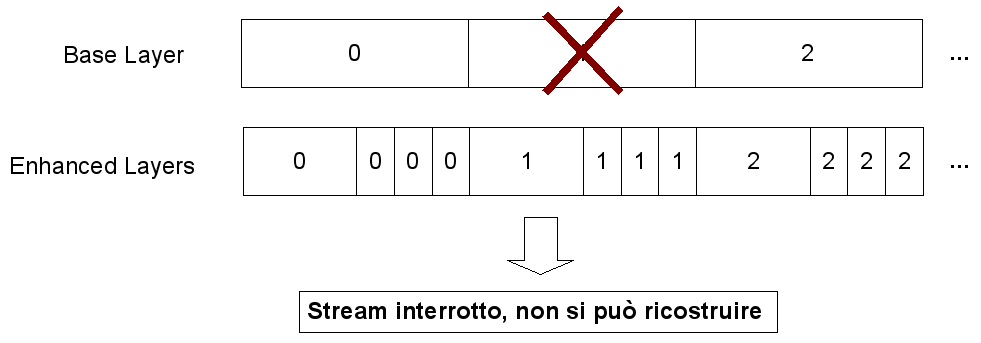
\includegraphics[width=0.90\textwidth]{../images/modello_layered_errori2.png}
\label{fig:modello_layered_errori2}
\caption{Modello Layered: perdita di un ``Base Layer''}
\end{figure}


\subsection{Modello \emph{Multiple Descriptions}}

Il Multiple Description Coding prevede che:
\begin{enumerate}
\item il flusso informativo sia suddiviso in più frammenti, detti 'Descrittori', con circa la stessa quantità di informazioni
\item i descrittori costituiscano due o più sotto-flussi;
\item i descrittori di un solo sotto-flusso, qualunque sia, devono essere
sufficienti per la ricostruzione dell'informazione, per lo meno con una bassa
qualità
\item se vengono ricevuti due o più sotto-flussi, la qualità dell'informazione decodificata aumenta 
\end{enumerate}

\begin{figure}[h]
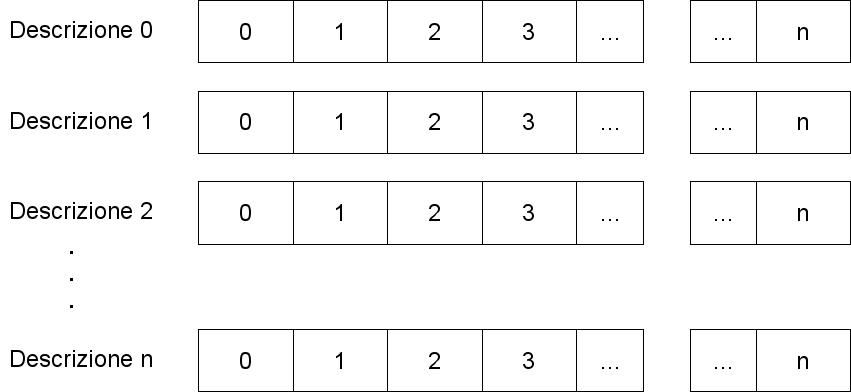
\includegraphics[width=0.90\textwidth]{../images/modello_mdc.png}
\label{fig:modello_mdc}
\caption{Modello Multiple Description Coding}
\end{figure}
\subsection{Differenze tra MDC e Layered}

La principale differenza tra la tipologia di codifica 'a descrizioni multiple' e
quella 'a strati' sta nella differente organizzazione delle informazioni: i
frammenti ottenuti con una codifica MDC hanno potenzialmente lo stesso contenuto
informativo in termini di quantità, mentre nei codec 'layered' esiste un
frammento 'base', più importante degli altri, e diversi frammenti più piccoli di
'avanzamento'.

\section{Obiettivi del sistema}

I principali obiettivi sono:

\begin{itemize}
\item progettazione e implementazione dei vari codec in un formato mdc-compatibile
\item progettazione e implementazione di un protocollo per lo scambio dei
flussi di dati in modo \emph{peer-to-peer} (chiamato MDSP)
\item implementazione di una piattaforma per il test del sistema
\end{itemize}






\section{Testbed}



\subsection{Organizzazione}


Il testbed è composto da un insieme di classi, suddivise per tipologia:



\begin{itemize}
\item \emph{common}: classi che facilitano la realizzazione delle proprie
applicazioni; comprendono utility per accedere alla rete, per simulare un comportamento multi-tasking, e altro.

\item \emph{codecs}: contiene sia classi astratte, da usare come base per i
codec reali, sia classi di utilità, come il registro dei codec, utilizzato per auto-caricare il codec adatto a seconda del flusso informativo

\item \emph{messages}: l'insieme dei messagi di base
\item \emph{app}: una applicazione client-server di esempio
\end{itemize}




\subsection{Implementazione}


Il testbed è stato sviluppato in C/C++, anche se, seguendo le specifiche del
protocollo, è possibile implementare una qualunque parte del sistema con
qualsiasi linguaggio. Come dimostrazione è stato sviluppato un client in
python, che ha come scopo principale l'uso della piattaforma su dispositivi
mobili (come Symbian e Windows Mobile).








